\documentclass{article}
\usepackage[letterpaper, margin=2cm]{geometry}
\usepackage[utf8]{inputenc}
\usepackage{hyperref}
\usepackage{pdflscape}
\usepackage[spanish]{babel}
\usepackage{enumerate}
\spanishdecimal{.}
\usepackage{url}
\usepackage{lscape}
\usepackage[normalem]{ulem}
\usepackage{cancel}
\usepackage{float}
\usepackage{graphicx}
\usepackage{booktabs}
\usepackage{algorithm}
\usepackage{algpseudocode}
\usepackage{bm}
\usepackage{amsmath}
\usepackage{multicol}
\usepackage{subcaption}
\usepackage[table,xcdraw]{xcolor}
\usepackage{setspace}
\usepackage{vmargin}
\usepackage{listings}
\usepackage{cite}
\definecolor{codegray}{rgb}{0.5,0.5,0.5}
\definecolor{backcolour}{rgb}{0.27,0.27,0.27}
\lstdefinestyle{mystyle}{
    backgroundcolor=\color{backcolour},   
    commentstyle=\color{green},
    keywordstyle=\color{yellow},
    numberstyle=\color{codegray},
    stringstyle=\color{pink},
    basicstyle=\color{white}\ttfamily\normalsize,
    breakatwhitespace=false,         
    breaklines=true,                 
    captionpos=b,                    
    keepspaces=true,                 
    numbers=left,                    
    numbersep=5pt,                  
    showspaces=false,                
    showstringspaces=false,
    showtabs=false,                  
    tabsize=2
}
\lstset{style=mystyle}
\renewcommand\ULthickness{1.3pt}   %%---> For changing thickness of underline
\setlength\ULdepth{1.9ex}






\begin{document}
	\noindent
	\begin{minipage}[l]{0.1\textwidth}
		\noindent
		
\includegraphics[width=1.1\textwidth]{imagenes/cimat_png.png}
	\end{minipage}
\hfill
\begin{minipage}[c]{0.8\textwidth}{
		Isaac Mauricio López Bocanegra \hfill 6/6/2026 \par
		mauricio.lopez@cimat.mx\hfill Optimización estocástica \par
        Maestría en ciencias de la computación \hfill Cubículo D-406-D\par}
\end{minipage}
\par
\vspace{0.2in}
\noindent

%%%%%% EDITAR AQUI %%%%%%
\uline{\hfill Proyecto\hfill}

\section{Introducción}

El Sudoku es un problema combinatorio de restricciones en el que se busca completar una cuadrícula o tablero parcialmente lleno respetando un conjunto de reglas. En su versión clásica, el tablero tiene tamaño \(9 \times 9\), dividido en nueve bloques de \(3 \times 3\). El objetivo es asignar un valor a cada casilla vacía tal que cada número aparezca exactamente una vez en cada fila, en cada columna y en cada bloque. Además, los valores dados inicialmente por la instancia, llamados pistas, no pueden modificarse.

Aunque Sudoku es conocido principalmente como un juego lógico, desde el punto de vista computacional puede formularse como un problema de optimización combinatoria, con restricciones. La dificultad surge porque el número de posibles asignaciones crece rápidamente con el tamaño del tablero y con el número de casillas vacías. Por eso el problema resulta práctico como caso de estudio para evaluar algoritmos metaheurísticos, en especial cuando se trabaja con instancias difíciles, con pocas pistas o con variantes mas grandes del tablero.

En este proyecto se aborda el problema de resolver instancias de Sudoku mediante técnicas de optimización estocástica. En lugar de aplicar un método exacto de retroceso o propagación de restricciones, se propone transformar el problema en la minimización de una función de penalización. Así, una solución candidata puede no ser necesariamente un Sudoku válido, pero su calidad se mide de acuerdo con el número de restricciones violadas. Una solución óptima corresponde a un tablero con penalización cero.

Sea \(n\) el tamaño de cada bloque del Sudoku. Entonces el tablero completo tiene dimensión \(n^2 \times n^2\), y los valores permitidos pertenecen al conjunto
\[
S = \{1,2,\ldots,n^2\}.
\]

Una solución candidata se representa como una matriz
\[
X = (x_{ij}), \qquad x_{ij} \in S,
\]
donde \(x_{ij}\) es el valor asignado a la casilla ubicada en la fila \(i\) y columna \(j\). Para las casillas fijas de la instancia original se impone la restricción
\[
x_{ij} = p_{ij},
\]
donde \(p_{ij}\) representa la pista dada en la posición \((i,j)\).

El Sudoku resuelto debe cumplir tres tipos de restricciones. Primero, cada fila debe contener todos los valores de \(S\) exactamente una vez. Segundo, cada columna debe cumplir la misma condición. Finalmente, cada bloque de tamaño \(n \times n\) también debe contener todos los valores una sola vez. Formalmente, para todo valor \(k \in S\), debe cumplirse:
\[
\sum_{j=1}^{n^2} \mathbf{1}(x_{ij}=k) = 1, \qquad \forall i,
\]
\[
\sum_{i=1}^{n^2} \mathbf{1}(x_{ij}=k) = 1, \qquad \forall j,
\]
y
\[
\sum_{(i,j)\in B_b} \mathbf{1}(x_{ij}=k) = 1, \qquad \forall b,
\]
donde \(B_b\) representa el conjunto de casillas que pertenecen al bloque \(b\).

Para resolver el problema mediante metaheurísticas, se define una función objetivo basada en penalizaciones por valores faltantes y repetidos. En este trabajo se consideran dos funciones de evaluación. La primera penaliza explícitamente los valores faltantes y sobrantes en filas, columnas y bloques. La segunda utiliza una formulación tipo QUBO, en la que se penaliza la desviación cuadrática respecto a la condición de que cada valor aparezca exactamente una vez en cada unidad del Sudoku. En ambos casos, el problema se plantea como
\[
\min f(X),
\]
donde \(f(X)=0\) si y solo si \(X\) corresponde a una solución válida del Sudoku.

Para explorar el espacio de soluciones se implementaron dos enfoques principales: recocido simulado y un algoritmo memético. El recocido simulado permite aceptar ocasionalmente soluciones peores con una probabilidad controlada por una temperatura, lo que ayuda a escapar de óptimos locales. Por otro lado, el algoritmo memético combina una estrategia poblacional con operadores de cruce, mutación y búsqueda local, buscando aprovechar tanto la exploración global de una población como la mejora intensiva de soluciones individuales.

El objetivo del proyecto es comparar el comportamiento de estas estrategias sobre diferentes conjuntos de instancias de Sudoku, analizando la calidad de las soluciones obtenidas, la estabilidad de los métodos y su capacidad para alcanzar soluciones factibles bajo restricciones de tiempo computacional.\\
\uline{\hfill \phantom{-} \hfill}
\section{Estado del arte}

El Sudoku se ha estudiado desde distintos enfoques computacionales porque puede verse como un problema de satisfacción de restricciones y también como un problema de optimización combinatoria. Aunque muchas instancias clásicas pueden resolverse con métodos exactos o técnicas de propagación de restricciones, las variantes más difíciles, los tableros generalizados y las instancias con pocas pistas siguen siendo útiles para evaluar algoritmos heurísticos y metaheurísticos.

Uno de los trabajos más representativos es el de Lewis, donde se muestra que las metaheurísticas pueden resolver Sudokus al plantear el problema como la minimización de una función de penalización. Bajo este enfoque, un tablero válido corresponde a una solución con penalización cero, idea que también se utiliza en este proyecto al evaluar conflictos en filas, columnas y bloques \cite{lewis2007metaheuristics}.

También se han aplicado variantes de recocido simulado, incluyendo versiones paralelas, debido a que este método puede escapar de óptimos locales al aceptar soluciones peores con cierta probabilidad \cite{karimi2010parallel}. Este enfoque se relaciona con el presente trabajo, donde se implementa recocido simulado y se ejecutan corridas independientes en paralelo mediante OpenMP.

Por otro lado, los algoritmos genéticos y meméticos han sido usados para resolver Sudoku mediante poblaciones de soluciones candidatas. Sin embargo, en instancias difíciles, un algoritmo genético simple puede perder diversidad o estancarse. Por ello, algunos trabajos resaltan la importancia de combinar operadores evolutivos con búsqueda local y mecanismos para preservar diversidad \cite{segura2016diversity}. En este proyecto se sigue esta idea mediante un algoritmo memético con cruce, mutación por intercambios válidos, renovación parcial de la población y búsqueda local tipo hill climbing.

Finalmente, también existen enfoques híbridos y formulaciones alternativas, como Iterated Local Search con programación por restricciones, Ant Colony Optimization y modelos tipo QUBO \cite{musliu2017hybrid,lloyd2019aco,zhao2025quantum}. Estas ideas muestran que Sudoku es un problema adecuado para estudiar codificaciones, vecindarios y funciones de penalización. Con base en estos antecedentes, este trabajo compara recocido simulado y un algoritmo memético para reducir las violaciones de restricciones y encontrar soluciones válidas.\\
\uline{\hfill \phantom{-} \hfill}
\section{Modelo de optimización}

En este proyecto, el Sudoku se modela como un problema de minimización. Cada solución candidata representa un tablero completo, donde las pistas originales se mantienen fijas y las casillas vacías se rellenan con valores candidatos. La idea es medir qué tan lejos está un tablero de ser una solución válida mediante una función de penalización. Por lo tanto, resolver el Sudoku equivale a encontrar un tablero con fitness igual a cero.

\subsection{Codificación}

Sea \(n\) el tamaño de los bloques del Sudoku. Entonces el tablero tiene dimensión \(n^2 \times n^2\), y los valores permitidos pertenecen al conjunto

\[
S = \{1,2,\ldots,n^2\}.
\]

Una solución candidata se representa como una matriz

\[
X = (x_{ij}), \qquad x_{ij}\in S,
\]

donde \(x_{ij}\) es el valor asignado a la casilla \((i,j)\). En la implementación, los valores se almacenan internamente como enteros de \(0\) a \(n^2-1\).

La codificación permite trabajar con tres representaciones: por filas, por columnas y por celdas. En la representación por filas, cada fila se inicializa como una permutación válida de los valores permitidos, respetando las pistas. De esta forma, las filas ya cumplen la estructura básica del Sudoku y la búsqueda se concentra en corregir conflictos en columnas y bloques. De manera similar, la representación por columnas preserva inicialmente la validez de las columnas.

Las pistas se guardan en una matriz de posiciones fijas, de modo que los operadores de búsqueda solo pueden modificar las casillas libres.
 
\subsection{Función objetivo}

Para evaluar una solución, se usan penalizaciones por valores faltantes y repetidos en filas, columnas y bloques. Sea \(U\) una unidad del tablero, es decir, una fila, columna o bloque, y sea \(c_U(k)\) el número de veces que aparece el valor \(k\) en esa unidad. La penalización usada es

\[
P(U)=
\sum_{k\in S}
\left[
w_1\mathbf{1}(c_U(k)=0)
+
w_2c_U(k)\mathbf{1}(c_U(k)>1)
\right],
\]

donde \(w_1\) penaliza valores faltantes y \(w_2\) penaliza valores repetidos. Entonces la función objetivo general es

\[
f(X)=
\sum_i P(F_i)
+
\sum_j P(C_j)
+
\sum_b P(B_b).
\]

También se implementó una segunda función tipo QUBO, en la que se penaliza de forma cuadrática la desviación respecto a que cada valor aparezca exactamente una vez en cada fila, columna y bloque. En ambos casos, el objetivo es

\[
\min f(X),
\]

donde \(f(X)=0\) indica que el Sudoku está resuelto.

\subsection{Vecindarios}

Los vecindarios se construyen mediante intercambios entre posiciones no fijas. El vecindario más pequeño consiste en elegir una fila, columna o unidad de la representación y hacer un solo intercambio entre dos casillas libres:

\[
x_{u,a} \leftrightarrow x_{u,b}.
\]

Este movimiento conserva las pistas originales y permite hacer cambios locales pequeños.

El segundo vecindario consiste en aplicar varios intercambios válidos consecutivos sobre el mismo tablero. Si se realizan \(q\) intercambios, el vecino queda definido como

\[
X' = \text{swap}_q(\cdots \text{swap}_2(\text{swap}_1(X))).
\]

Este vecindario genera perturbaciones más grandes y se usa tanto en el recocido simulado como en el algoritmo memético. En el recocido, el número de intercambios se controla con el parámetro \texttt{N swaps}; en el algoritmo memético, también se usa como mutación mediante \texttt{N swaps cambio}.

En todos los casos, los movimientos respetan las pistas originales y mantienen parcialmente la estructura de la solución. Esto reduce el espacio de búsqueda y evita generar tableros completamente arbitrarios.

\subsection{Algoritmo memético}

El algoritmo memético es la propuesta principal de este trabajo. La idea es combinar un algoritmo poblacional con una búsqueda local, de modo que la población permita explorar distintas regiones del espacio de soluciones, mientras que la búsqueda local mejore cada individuo de forma más intensiva.

El método inicia con una población de tableros completos generados aleatoriamente, respetando siempre las pistas originales. En cada iteración, la población se ordena por fitness y se seleccionan los mejores individuos como padres. A partir de ellos se generan nuevos individuos mediante operadores de cruce. Después, se aplica una mutación basada en intercambios válidos entre posiciones no fijas.

Cada nuevo individuo se mejora con una búsqueda local tipo hill climbing. Esta búsqueda intenta intercambios aleatorios y conserva el cambio si el fitness no empeora. Finalmente, los nuevos individuos compiten contra la población anterior mediante reemplazo. Para mantener diversidad, cada cierto número de iteraciones se renueva la peor mitad de la población con individuos nuevos.

\begin{algorithm}[H]
\caption{Algoritmo memético propuesto}
\begin{algorithmic}[1]
\Require Instancia de Sudoku, población \(N\), padres \(N_p\), iteraciones \(I\)
\Ensure Mejor tablero encontrado
\State Inicializar población \(P\) respetando las pistas
\For{\(t=1\) hasta \(I\)}
    \State Ordenar \(P\) por fitness
    \State Seleccionar los \(N_p\) mejores individuos como padres
    \For{\(i=1\) hasta \(N\)}
        \State Elegir dos padres aleatoriamente
        \State Generar hijo mediante cruce
        \State Aplicar mutación por intercambios válidos
        \State Mejorar hijo con búsqueda local
    \EndFor
    \State Reemplazar individuos mediante torneo
    \If{\(t\) es múltiplo de \(I_r\)}
        \State Renovar la peor mitad de la población
    \EndIf
    \If{se excede el tiempo límite}
        \State Detener ejecución
    \EndIf
\EndFor
\State \Return mejor individuo de \(P\)
\end{algorithmic}
\end{algorithm}

\subsubsection{Complejidad del algoritmo memético}

Sea \(N\) el número de individuos, \(I\) el número de iteraciones y \(M=n^2\) el tamaño lateral del tablero. En cada iteración se ordena la población y se generan \(N\) nuevos individuos. Además, cada hijo se evalúa y se mejora mediante búsqueda local.

La evaluación básica del fitness recorre filas, columnas y bloques, por lo que tiene costo aproximado

\[
O(M^2).
\]

Si la búsqueda local realiza hasta \(s\) intentos consecutivos sin mejora, el costo aproximado por iteración es

\[
O(N\log N + NsM^2).
\]

Por lo tanto, la complejidad total del algoritmo memético puede expresarse como

\[
O\left(I(N\log N + NsM^2)\right).
\]

Esta estimación considera la función de fitness basada en faltantes y repetidos. En el caso de la evaluación tipo QUBO, el costo de evaluación es mayor, por lo que el término \(M^2\) puede sustituirse por \(M^3\).

\subsection{Recocido simulado}

El recocido simulado se implementó como método de comparación y sigue la forma clásica del algoritmo. A diferencia del algoritmo memético, este método trabaja con una solución a la vez. A partir de un tablero inicial, se generan vecinos mediante intercambios válidos entre posiciones no fijas, respetando siempre las pistas originales.

Si el vecino mejora el fitness, se acepta directamente. Si empeora la solución, todavía puede aceptarse con una probabilidad que depende de la temperatura actual. Esta probabilidad se define como

\[
P(\text{aceptar}) = \exp\left(-\frac{\Delta}{T}\right),
\]

donde

\[
\Delta = f(X') - f(X)
\]

es el cambio en el fitness, \(X\) es la solución actual, \(X'\) es el vecino generado y \(T\) es la temperatura actual. Al inicio, cuando la temperatura es alta, el algoritmo acepta con mayor facilidad movimientos que empeoran la solución. Esto ayuda a escapar de óptimos locales. Conforme la temperatura disminuye, el método se vuelve más selectivo.

\begin{algorithm}[H]
\caption{Recocido simulado}
\begin{algorithmic}[1]
\Require Solución inicial \(X\), temperatura inicial \(T_0\), temperatura final \(T_f\), factor de enfriamiento \(\alpha\)
\Ensure Mejor solución encontrada
\State \(X_{\text{actual}} \gets X\)
\State \(X_{\text{mejor}} \gets X\)
\State \(T \gets T_0\)
\While{\(T>T_f\)}
    \State Generar vecino \(X'\) mediante intercambios válidos
    \State \(\Delta \gets f(X') - f(X_{\text{actual}})\)
    \If{\(\Delta \leq 0\)}
        \State \(X_{\text{actual}} \gets X'\)
    \Else
        \State Aceptar \(X'\) con probabilidad \(\exp(-\Delta/T)\)
    \EndIf
    \If{\(f(X_{\text{actual}})<f(X_{\text{mejor}})\)}
        \State \(X_{\text{mejor}} \gets X_{\text{actual}}\)
    \EndIf
    \State \(T \gets \alpha T\)
    \If{se excede el tiempo límite}
        \State Detener ejecución
    \EndIf
\EndWhile
\State \Return \(X_{\text{mejor}}\)
\end{algorithmic}
\end{algorithm}

\subsubsection{Complejidad del recocido simulado}

Sea \(M=n^2\) el tamaño lateral del tablero. La evaluación básica del fitness recorre filas, columnas y bloques, por lo que tiene costo aproximado

\[
O(M^2).
\]

Si \(L\) es el número de temperaturas evaluadas durante el enfriamiento, entonces una corrida de recocido simulado tiene complejidad aproximada

\[
O(LM^2).
\]

En la implementación se ejecutan \(N\) soluciones iniciales independientes, por lo que el costo total puede expresarse como

\[
O(NLM^2).
\]

Si se usa la función de evaluación tipo QUBO, el costo de evaluación aumenta y el término \(M^2\) puede sustituirse por \(M^3\).\\
\uline{\hfill \phantom{-} \hfill}
\section{Diseño experimental}

El objetivo de los experimentos fue comparar el desempeño del recocido simulado y del algoritmo memético sobre instancias públicas de Sudoku. Para que la comparación fuera justa, ambas técnicas se ejecutaron sobre los mismos conjuntos de instancias y bajo el mismo número de repeticiones independientes.

\subsection{Datasets utilizados}

Se utilizaron dos conjuntos de instancias tomados de la literatura. El primero corresponde a las instancias reportadas en el trabajo de Ant Colony Optimization para Sudoku. De este conjunto se utilizaron únicamente las instancias del grupo \textit{logic solved}, reportadas en la Tabla 4 de dicho artículo \cite{lloyd2019aco}. Este conjunto resulta útil porque contiene Sudokus que pueden resolverse mediante técnicas lógicas, pero que aun así permiten evaluar el comportamiento de las metaheurísticas.

El segundo conjunto de instancias fue tomado del trabajo \textit{The importance of diversity in the application of evolutionary algorithms to the Sudoku problem} \cite{segura2016diversity}. En este caso se utilizaron todas las instancias disponibles, ya que el artículo está directamente relacionado con algoritmos evolutivos aplicados a Sudoku y con la importancia de mantener diversidad dentro de la población.

En total, los experimentos se organizaron en tres grupos de datos dentro de la implementación:

\begin{itemize}
    \item \texttt{General}: instancias generales tomadas de la literatura.
    \item \texttt{Solvable}: instancias del conjunto \textit{logic solved}.
    \item \texttt{SudokuPuzzles}: conjunto de instancias adicionales usadas para ampliar la evaluación.
\end{itemize}

Cada instancia fue leída desde archivo, almacenando por separado las pistas originales y las posiciones modificables. De esta forma, todos los algoritmos trabajaron con la misma representación de restricciones.

\subsection{Configuración experimental}

Cada instancia fue resuelta mediante las dos técnicas implementadas: recocido simulado y algoritmo memético. Para cada combinación de instancia y algoritmo se realizaron 30 corridas independientes. En cada corrida se utilizó una semilla diferente, generada a partir de una semilla base más el índice del experimento. Esto permitió observar no solo el mejor resultado obtenido, sino también la estabilidad de cada método.

Los experimentos se ejecutaron con una restricción de tiempo por corrida. Además, las corridas independientes se paralelizaron usando OpenMP, asignando el número de hilos indicado en el archivo de configuración de cada experimento.

\begin{table}[H]
\centering
\caption{Parámetros generales de los experimentos.}
\begin{tabular}{ll}
\hline
Parámetro & Valor \\
\hline
Número de corridas por instancia & 30 \\
Algoritmos comparados & Memético y recocido simulado \\
Paralelización & OpenMP \\
Semillas & \texttt{Seed + índice de corrida} \\
Restricción de tiempo & \texttt{Restriccion tiempo} segundos \\
Función de fitness & Faltantes/sobrantes o QUBO \\
Representación & Filas, columnas o celdas \\
\hline
\end{tabular}
\end{table}

\subsection{Parámetros de los algoritmos}

Para el algoritmo memético, como se puede ver en la tabla \ref{tab:params} se consideraron parámetros relacionados con el tamaño de la población, el número de padres, el tipo de cruce, la cantidad de intercambios usados como mutación y el número máximo de iteraciones. Además, se incluyó una renovación parcial de la población cada cierto número de iteraciones, reemplazando la peor mitad por individuos nuevos.
\begin{table}[H]
\centering
\caption{Parámetros del algoritmo memético.}
\label{tab:params}
\begin{tabular}{ll}
\hline
Parámetro & Descripción \\
\hline
\texttt{N inds} & Tamaño de la población \\
\texttt{N padres} & Número de padres seleccionados \\
\texttt{N its} & Número máximo de iteraciones \\
\texttt{Crossover} & Cruce binario o cruce de dos cortes \\
\texttt{N swaps cambio} & Intercambios usados como mutación \\
\texttt{N swaps} & Intentos sin mejora en la búsqueda local \\
\texttt{n\_iters\_renovacion} & Frecuencia de renovación poblacional \\
\hline
\end{tabular}
\end{table}

Para el recocido simulado, como se puede ver en la tabla \ref{tab:__}, se utilizaron los parámetros clásicos del método: temperatura inicial, temperatura final, factor de enfriamiento y número de intercambios usados para generar cada vecino.

\begin{table}[H]
\centering
\caption{Parámetros del recocido simulado.}
\label{tab:__}
\begin{tabular}{ll}
\hline
Parámetro & Descripción \\
\hline
\texttt{N inds} & Número de soluciones iniciales independientes \\
\texttt{Temp inicial} & Temperatura inicial \\
\texttt{Temp final} & Temperatura mínima de parada \\
\texttt{Cambio} & Factor de enfriamiento \\
\texttt{N swaps} & Intercambios usados para generar vecinos \\
\hline
\end{tabular}
\end{table}

\subsection{Métricas de evaluación}

Para cada corrida se guardaron los resultados en archivos \texttt{JSON}. Las métricas registradas fueron:

\begin{itemize}
    \item mejor fitness encontrado,
    \item peor fitness de la población final,
    \item fitness promedio,
    \item desviación estándar del fitness.
\end{itemize}

La métrica principal fue el mejor fitness encontrado, ya que un valor de cero indica que el Sudoku fue resuelto correctamente. Además, el promedio y la desviación estándar permitieron analizar la estabilidad de cada algoritmo a lo largo de las 30 corridas independientes.

Finalmente, los resultados fueron agrupados por instancia, dataset y algoritmo, para generar tablas comparativas y gráficas tipo boxplot. Estas visualizaciones permiten comparar tanto la calidad de las soluciones como la variabilidad de los métodos.\\
\uline{\hfill \phantom{-} \hfill}
\section{Resultados}
La Tabla~\ref{tab:kw_general} presenta la comparación global entre el algoritmo memético y el recocido simulado mediante la prueba de Kruskal-Wallis. Como el valor de \(p\) es menor que \(0.05\), existe una diferencia estadísticamente significativa entre ambos métodos. Además, la mediana del fitness es menor para el memético, por lo que este obtuvo mejores resultados generales.\begin{table}
\caption{Prueba de Kruskal-Wallis general entre algoritmos}
\label{tab:kw_general}
\begin{tabular}{lrrrrl}
\toprule
Comparación & H & p-value & Mediana memético & Mediana recocido & Mejor algoritmo \\
\midrule
General & 1799.508 & 0.000 & 0.111 & 0.885 & memetico \\
\bottomrule
\end{tabular}
\end{table}

La Tabla~\ref{tab:kw_dataset} muestra la comparación entre algoritmos separada por dataset. En ambos casos, el valor de \(p\) es menor que \(0.05\), por lo que existen diferencias estadísticamente significativas. Además, las medianas del fitness son menores para el algoritmo memético tanto en \textit{logic} como en \textit{puzzles}, indicando un mejor desempeño en ambos conjuntos.
\begin{table}
\caption{Prueba de Kruskal-Wallis por dataset.}
\label{tab:kw_dataset}
\begin{tabular}{lrrrrl}
\toprule
Dataset & H & p-value & Mediana memético & Mediana recocido & Mejor algoritmo \\
\midrule
logic & 674.9450 & 0.0000 & 0.0667 & 0.8462 & memetico \\
puzzles & 1124.2335 & 0.0000 & 0.1200 & 0.8889 & memetico \\
\bottomrule
\end{tabular}
\end{table}

La Tabla~\ref{tab:conteo_ganadores} resume el número de instancias en las que cada algoritmo obtuvo el mejor resultado. En ambos datasets, todas las instancias fueron ganadas por el algoritmo memético: 15 en \textit{logic} y 25 en \textit{puzzles}. Esto refuerza lo observado en las pruebas anteriores, donde el memético mostró un desempeño más consistente que el recocido simulado.

\begin{table}
\caption{Conteo de instancias ganadas por algoritmo.}
\label{tab:conteo_ganadores}
\begin{tabular}{llr}
\toprule
dataset & Ganador & Número de instancias \\
\midrule
logic & memetico & 15 \\
puzzles & memetico & 25 \\
\bottomrule
\end{tabular}
\end{table}

Las Figuras~\ref{fig:comparacion_general} y~\ref{fig:comparacion_dataset} muestran la distribución del fitness normalizado para los algoritmos evaluados. En la comparación general, el algoritmo memético obtiene valores claramente menores que el recocido simulado, con una mediana cercana a cero. Al separar los resultados por dataset, se observa el mismo comportamiento en \textit{logic} y \textit{puzzles}, lo que confirma que el memético tuvo un desempeño más consistente y de mejor calidad en las instancias analizadas.

\begin{figure}[H]
    \centering
    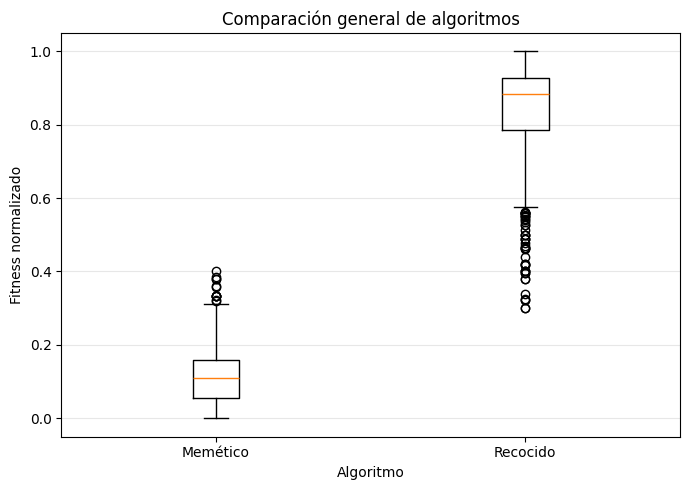
\includegraphics[width=0.75\textwidth]{imagenes/generales.png}
    \caption{Comparación general del fitness normalizado entre el algoritmo memético y el recocido simulado.}
    \label{fig:comparacion_general}
\end{figure}
\begin{figure}[H]
    \centering
    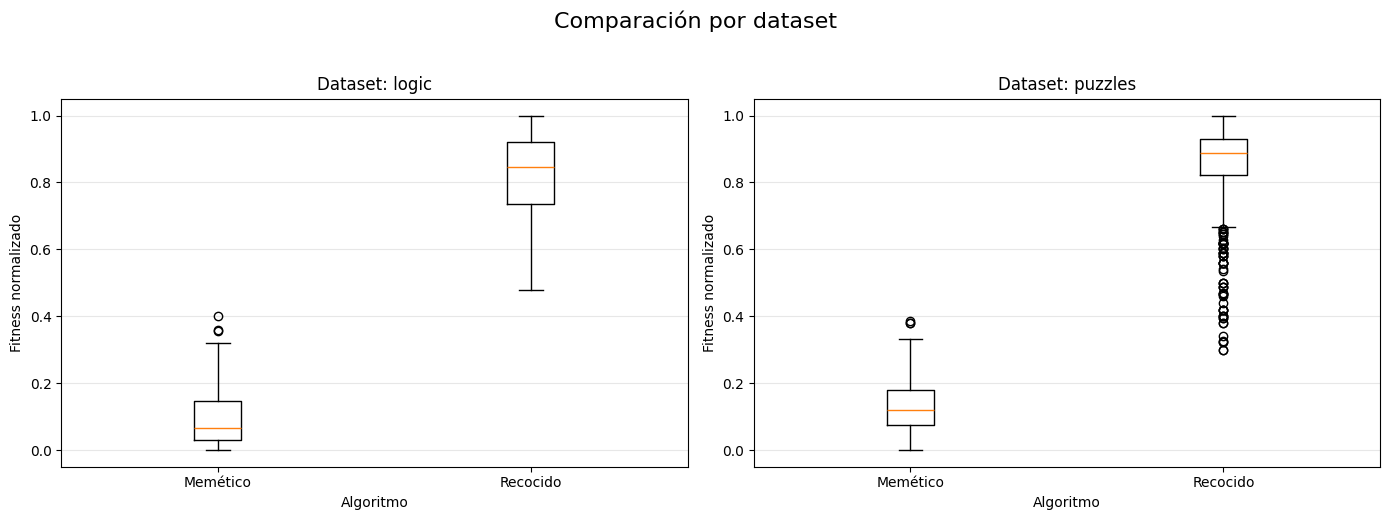
\includegraphics[width=\textwidth]{imagenes/datasets.png}
    \caption{Comparación del fitness normalizado por dataset para el algoritmo memético y el recocido simulado.}
    \label{fig:comparacion_dataset}
\end{figure}

La Tabla~\ref{tab:comparacion_acs_bve_instancia} compara los resultados obtenidos por el algoritmo memético y el recocido simulado contra los valores reportados por Lloyd y Amos para ACS+BVE. En todas las instancias, ACS+BVE alcanza una tasa de éxito del \(100\%\), por lo que sigue siendo superior como método especializado. Sin embargo, entre los dos métodos implementados en este trabajo, el algoritmo memético obtiene consistentemente mejores valores de fitness que el recocido simulado. Además, logra resolver algunas instancias, como \textit{reddwarf}, \textit{sabuncu1}, \textit{sabuncu10} y \textit{sabuncu4}, mientras que el recocido no alcanza éxito en ninguna de las corridas.
\begin{table}[H]
\centering
\caption{Comparación por instancia contra MULTI DYN reportado por Segura et al.}
\label{tab:comparacion_multi_dyn_instancia}
\resizebox{\textwidth}{!}{
\begin{tabular}{rllrrrrrrr}
\toprule
Instancia & Instancia paper & Algoritmo & Media & Desviacion & Mejor & Peor & Success rate (\%) & MULTI\_DYN Success rate (\%) & MULTI\_DYN Tiempo (s) \\
\midrule
1 & Film1 & memetico & 11.200 & 3.662 & 6.000 & 24.000 & 0.000 & 83.300 & 155.000 \\
1 & Film1 & recocido & 53.533 & 3.350 & 46.000 & 60.000 & 0.000 & 83.300 & 155.000 \\
2 & Film2 & memetico & 13.067 & 3.886 & 4.000 & 20.000 & 0.000 & 63.300 & 208.000 \\
2 & Film2 & recocido & 58.200 & 2.797 & 52.000 & 64.000 & 0.000 & 63.300 & 208.000 \\
3 & Inkala & memetico & 11.467 & 3.748 & 4.000 & 20.000 & 0.000 & 100.000 & 67.300 \\
3 & Inkala & recocido & 55.533 & 2.909 & 48.000 & 60.000 & 0.000 & 100.000 & 67.300 \\
4 & SD1 & memetico & 13.667 & 4.551 & 4.000 & 26.000 & 0.000 & 100.000 & 14.500 \\
4 & SD1 & recocido & 56.267 & 2.959 & 50.000 & 62.000 & 0.000 & 100.000 & 14.500 \\
5 & SD2 & memetico & 14.600 & 4.731 & 8.000 & 24.000 & 0.000 & 100.000 & 7.600 \\
5 & SD2 & recocido & 57.267 & 3.463 & 50.000 & 64.000 & 0.000 & 100.000 & 7.600 \\
6 & SD3 & memetico & 12.400 & 3.838 & 4.000 & 20.000 & 0.000 & 100.000 & 10.800 \\
6 & SD3 & recocido & 53.200 & 3.951 & 44.000 & 60.000 & 0.000 & 100.000 & 10.800 \\
7 & SS1 & memetico & 11.933 & 4.533 & 4.000 & 22.000 & 0.000 & 100.000 & 1.800 \\
7 & SS1 & recocido & 52.800 & 3.662 & 44.000 & 58.000 & 0.000 & 100.000 & 1.800 \\
8 & SS10 & memetico & 13.133 & 4.974 & 4.000 & 26.000 & 0.000 & 100.000 & 5.400 \\
8 & SS10 & recocido & 57.333 & 3.252 & 48.000 & 62.000 & 0.000 & 100.000 & 5.400 \\
9 & SS2 & memetico & 10.867 & 3.989 & 4.000 & 20.000 & 0.000 & 100.000 & 12.500 \\
9 & SS2 & recocido & 51.133 & 3.848 & 36.000 & 56.000 & 0.000 & 100.000 & 12.500 \\
10 & SS3 & memetico & 11.000 & 4.323 & 4.000 & 20.000 & 0.000 & 100.000 & 4.800 \\
10 & SS3 & recocido & 50.467 & 3.003 & 46.000 & 56.000 & 0.000 & 100.000 & 4.800 \\
11 & SS4 & memetico & 14.467 & 4.416 & 8.000 & 28.000 & 0.000 & 100.000 & 63.400 \\
11 & SS4 & recocido & 55.000 & 3.096 & 50.000 & 60.000 & 0.000 & 100.000 & 63.400 \\
12 & SS5 & memetico & 14.067 & 3.172 & 8.000 & 24.000 & 0.000 & 100.000 & 5.900 \\
12 & SS5 & recocido & 54.800 & 3.845 & 46.000 & 60.000 & 0.000 & 100.000 & 5.900 \\
13 & SS6 & memetico & 9.733 & 3.778 & 4.000 & 16.000 & 0.000 & 100.000 & 7.100 \\
13 & SS6 & recocido & 48.667 & 2.845 & 44.000 & 54.000 & 0.000 & 100.000 & 7.100 \\
14 & SS7 & memetico & 14.000 & 3.562 & 8.000 & 20.000 & 0.000 & 100.000 & 1.400 \\
14 & SS7 & recocido & 53.933 & 4.472 & 40.000 & 60.000 & 0.000 & 100.000 & 1.400 \\
15 & SS8 & memetico & 8.467 & 3.627 & 4.000 & 16.000 & 0.000 & 100.000 & 2.200 \\
15 & SS8 & recocido & 53.267 & 2.377 & 48.000 & 58.000 & 0.000 & 100.000 & 2.200 \\
16 & SS9 & memetico & 12.800 & 4.536 & 6.000 & 22.000 & 0.000 & 100.000 & 1.500 \\
16 & SS9 & recocido & 53.400 & 3.568 & 46.000 & 60.000 & 0.000 & 100.000 & 1.500 \\
17 & SW1 & memetico & 11.333 & 3.122 & 4.000 & 16.000 & 0.000 & 100.000 & 3.600 \\
17 & SW1 & recocido & 53.267 & 2.803 & 46.000 & 58.000 & 0.000 & 100.000 & 3.600 \\
18 & SW10 & memetico & 12.267 & 3.956 & 4.000 & 22.000 & 0.000 & 100.000 & 4.200 \\
18 & SW10 & recocido & 53.467 & 3.441 & 46.000 & 58.000 & 0.000 & 100.000 & 4.200 \\
19 & SW2 & memetico & 13.400 & 3.793 & 4.000 & 22.000 & 0.000 & 100.000 & 2.400 \\
19 & SW2 & recocido & 49.800 & 3.836 & 42.000 & 58.000 & 0.000 & 100.000 & 2.400 \\
20 & SW3 & memetico & 11.133 & 3.665 & 4.000 & 18.000 & 0.000 & 100.000 & 5.400 \\
20 & SW3 & recocido & 51.600 & 3.125 & 42.000 & 56.000 & 0.000 & 100.000 & 5.400 \\
21 & SW4 & memetico & 13.133 & 3.739 & 4.000 & 22.000 & 0.000 & 100.000 & 1.200 \\
21 & SW4 & recocido & 54.800 & 3.845 & 46.000 & 60.000 & 0.000 & 100.000 & 1.200 \\
22 & SW5 & memetico & 12.667 & 4.737 & 4.000 & 22.000 & 0.000 & 100.000 & 4.800 \\
22 & SW5 & recocido & 114.333 & 11.068 & 94.000 & 142.000 & 0.000 & 100.000 & 4.800 \\
23 & SW6 & memetico & 70.933 & 2.559 & 66.000 & 74.000 & 0.000 & 100.000 & 3.700 \\
23 & SW6 & recocido & 112.400 & 10.972 & 88.000 & 134.000 & 0.000 & 100.000 & 3.700 \\
24 & SW7 & memetico & 72.400 & 4.530 & 60.000 & 80.000 & 0.000 & 100.000 & 2.300 \\
24 & SW7 & recocido & 114.200 & 15.908 & 90.000 & 160.000 & 0.000 & 100.000 & 2.300 \\
25 & SW8 & memetico & 69.933 & 4.315 & 60.000 & 78.000 & 0.000 & 100.000 & 2.100 \\
25 & SW8 & recocido & 110.067 & 13.261 & 88.000 & 146.000 & 0.000 & 100.000 & 2.100 \\
\bottomrule
\end{tabular}
}
\end{table}

La Tabla~\ref{tab:comparacion_multi_dyn_instancia} compara los resultados obtenidos contra MULTI DYN, reportado por Segura et al. En este conjunto, el método de referencia obtiene tasas de éxito altas, en la mayoría de los casos del \(100\%\), por lo que sigue siendo superior a los métodos implementados en este trabajo. Sin embargo, al comparar únicamente el algoritmo memético y el recocido simulado, el memético obtiene mejores valores de fitness en todas las instancias. Esto confirma que la búsqueda poblacional con mejora local fue más efectiva que el recocido simulado canónico, aunque todavía no alcanza el desempeño del estado del arte.
\begin{landscape}
\begin{table}[p]
\centering
\scriptsize
\caption{Comparación por instancia contra ACS+BVE reportado por Lloyd y Amos.}
\label{tab:comparacion_acs_bve_instancia}
\resizebox{\linewidth}{!}{
\begin{tabular}{rllrrrrrrr}
\toprule
Instancia & Instancia paper & Algoritmo & Media & Desv. & Mejor & Peor & SR (\%) & ACS+BVE SR (\%) & ACS+BVE Tiempo (s) \\
\midrule
1 & Film1 & memetico & 11.200 & 3.662 & 6.000 & 24.000 & 0.000 & 83.300 & 155.000 \\
1 & Film1 & recocido & 53.533 & 3.350 & 46.000 & 60.000 & 0.000 & 83.300 & 155.000 \\
2 & Film2 & memetico & 13.067 & 3.886 & 4.000 & 20.000 & 0.000 & 63.300 & 208.000 \\
2 & Film2 & recocido & 58.200 & 2.797 & 52.000 & 64.000 & 0.000 & 63.300 & 208.000 \\
3 & Inkala & memetico & 11.467 & 3.748 & 4.000 & 20.000 & 0.000 & 100.000 & 67.300 \\
3 & Inkala & recocido & 55.533 & 2.909 & 48.000 & 60.000 & 0.000 & 100.000 & 67.300 \\
4 & SD1 & memetico & 13.667 & 4.551 & 4.000 & 26.000 & 0.000 & 100.000 & 14.500 \\
4 & SD1 & recocido & 56.267 & 2.959 & 50.000 & 62.000 & 0.000 & 100.000 & 14.500 \\
5 & SD2 & memetico & 14.600 & 4.731 & 8.000 & 24.000 & 0.000 & 100.000 & 7.600 \\
5 & SD2 & recocido & 57.267 & 3.463 & 50.000 & 64.000 & 0.000 & 100.000 & 7.600 \\
6 & SD3 & memetico & 12.400 & 3.838 & 4.000 & 20.000 & 0.000 & 100.000 & 10.800 \\
6 & SD3 & recocido & 53.200 & 3.951 & 44.000 & 60.000 & 0.000 & 100.000 & 10.800 \\
7 & SS1 & memetico & 11.933 & 4.533 & 4.000 & 22.000 & 0.000 & 100.000 & 1.800 \\
7 & SS1 & recocido & 52.800 & 3.662 & 44.000 & 58.000 & 0.000 & 100.000 & 1.800 \\
8 & SS10 & memetico & 13.133 & 4.974 & 4.000 & 26.000 & 0.000 & 100.000 & 5.400 \\
8 & SS10 & recocido & 57.333 & 3.252 & 48.000 & 62.000 & 0.000 & 100.000 & 5.400 \\
\bottomrule
\end{tabular}
}
\end{table}
\end{landscape}
\begin{landscape}

\begin{table}[p]
\centering
\scriptsize
\caption{Comparación por instancia contra ACS+BVE reportado por Lloyd y Amos (instancias 9--15).}
\label{tab:comparacion_acs_bve_instancia_2}
\resizebox{\linewidth}{!}{
\begin{tabular}{rllrrrrrrr}
\toprule
Inst. & Instancia paper & Algoritmo & Media & Desv. & Mejor & Peor & SR (\%) & ACS+BVE SR (\%) & ACS+BVE t (s) \\
\midrule
9 & SS2 & memetico & 10.867 & 3.989 & 4.000 & 20.000 & 0.000 & 100.000 & 12.500 \\
9 & SS2 & recocido & 51.133 & 3.848 & 36.000 & 56.000 & 0.000 & 100.000 & 12.500 \\
10 & SS3 & memetico & 11.000 & 4.323 & 4.000 & 20.000 & 0.000 & 100.000 & 4.800 \\
10 & SS3 & recocido & 50.467 & 3.003 & 46.000 & 56.000 & 0.000 & 100.000 & 4.800 \\
11 & SS4 & memetico & 14.467 & 4.416 & 8.000 & 28.000 & 0.000 & 100.000 & 63.400 \\
11 & SS4 & recocido & 55.000 & 3.096 & 50.000 & 60.000 & 0.000 & 100.000 & 63.400 \\
12 & SS5 & memetico & 14.067 & 3.172 & 8.000 & 24.000 & 0.000 & 100.000 & 5.900 \\
12 & SS5 & recocido & 54.800 & 3.845 & 46.000 & 60.000 & 0.000 & 100.000 & 5.900 \\
13 & SS6 & memetico & 9.733 & 3.778 & 4.000 & 16.000 & 0.000 & 100.000 & 7.100 \\
13 & SS6 & recocido & 48.667 & 2.845 & 44.000 & 54.000 & 0.000 & 100.000 & 7.100 \\
14 & SS7 & memetico & 14.000 & 3.562 & 8.000 & 20.000 & 0.000 & 100.000 & 1.400 \\
14 & SS7 & recocido & 53.933 & 4.472 & 40.000 & 60.000 & 0.000 & 100.000 & 1.400 \\
15 & SS8 & memetico & 8.467 & 3.627 & 4.000 & 16.000 & 0.000 & 100.000 & 2.200 \\
15 & SS8 & recocido & 53.267 & 2.377 & 48.000 & 58.000 & 0.000 & 100.000 & 2.200 \\
16 & SS9 & memetico & 12.800 & 4.536 & 6.000 & 22.000 & 0.000 & 100.000 & 1.500 \\
16 & SS9 & recocido & 53.400 & 3.568 & 46.000 & 60.000 & 0.000 & 100.000 & 1.500 \\
17 & SW1 & memetico & 11.333 & 3.122 & 4.000 & 16.000 & 0.000 & 100.000 & 3.600 \\
17 & SW1 & recocido & 53.267 & 2.803 & 46.000 & 58.000 & 0.000 & 100.000 & 3.600 \\
18 & SW10 & memetico & 12.267 & 3.956 & 4.000 & 22.000 & 0.000 & 100.000 & 4.200 \\
18 & SW10 & recocido & 53.467 & 3.441 & 46.000 & 58.000 & 0.000 & 100.000 & 4.200 \\
19 & SW2 & memetico & 13.400 & 3.793 & 4.000 & 22.000 & 0.000 & 100.000 & 2.400 \\
19 & SW2 & recocido & 49.800 & 3.836 & 42.000 & 58.000 & 0.000 & 100.000 & 2.400 \\
20 & SW3 & memetico & 11.133 & 3.665 & 4.000 & 18.000 & 0.000 & 100.000 & 5.400 \\
20 & SW3 & recocido & 51.600 & 3.125 & 42.000 & 56.000 & 0.000 & 100.000 & 5.400 \\
21 & SW4 & memetico & 13.133 & 3.739 & 4.000 & 22.000 & 0.000 & 100.000 & 1.200 \\
21 & SW4 & recocido & 54.800 & 3.845 & 46.000 & 60.000 & 0.000 & 100.000 & 1.200 \\
22 & SW5 & memetico & 12.667 & 4.737 & 4.000 & 22.000 & 0.000 & 100.000 & 4.800 \\
22 & SW5 & recocido & 114.333 & 11.068 & 94.000 & 142.000 & 0.000 & 100.000 & 4.800 \\
23 & SW6 & memetico & 70.933 & 2.559 & 66.000 & 74.000 & 0.000 & 100.000 & 3.700 \\
23 & SW6 & recocido & 112.400 & 10.972 & 88.000 & 134.000 & 0.000 & 100.000 & 3.700 \\
24 & SW7 & memetico & 72.400 & 4.530 & 60.000 & 80.000 & 0.000 & 100.000 & 2.300 \\
24 & SW7 & recocido & 114.200 & 15.908 & 90.000 & 160.000 & 0.000 & 100.000 & 2.300 \\
25 & SW8 & memetico & 69.933 & 4.315 & 60.000 & 78.000 & 0.000 & 100.000 & 2.100 \\
25 & SW8 & recocido & 110.067 & 13.261 & 88.000 & 146.000 & 0.000 & 100.000 & 2.100 \\
\bottomrule
\end{tabular}
}
\end{table}
\end{landscape}
\section{Conclusiones}
En este proyecto se abordó el problema de resolver Sudokus como un problema de optimización combinatoria con restricciones. Para ello, se transformó el problema en la minimización de una función de penalización, donde un fitness igual a cero representa una solución válida del Sudoku. Bajo este enfoque se implementaron y compararon dos métodos estocásticos: recocido simulado y un algoritmo memético.

Los resultados muestran que el algoritmo memético tuvo un desempeño claramente superior al recocido simulado. Esto se observó tanto en las pruebas estadísticas de Kruskal-Wallis como en las gráficas tipo boxplot y en el conteo de instancias ganadas. En particular, el memético obtuvo menores valores de fitness en todos los conjuntos evaluados, lo que indica que la combinación de búsqueda poblacional, cruce, mutación y mejora local fue más efectiva que una búsqueda trayectorial basada únicamente en recocido simulado.

Una posible explicación de este comportamiento es que el algoritmo memético mantiene una mejor exploración del espacio de soluciones gracias a la población, mientras que la búsqueda local permite mejorar de manera intensiva cada individuo. Además, la renovación periódica de la peor mitad de la población ayudó a mantener diversidad y a reducir el estancamiento en regiones poco prometedoras. En cambio, el recocido simulado, al trabajar con una solución a la vez, mostró mayor dificultad para acercarse a soluciones factibles en las instancias más complicadas.

Al comparar contra los métodos reportados en la literatura, como ACS+BVE y MULTI DYN, se observa que los métodos especializados siguen teniendo un mejor desempeño, especialmente en términos de tasa de éxito. Sin embargo, los resultados obtenidos permiten identificar que la propuesta memética es una base prometedora, ya que logró acercarse mucho más a soluciones válidas que el recocido simulado e incluso resolvió algunas instancias del conjunto evaluado.

Como trabajo futuro, sería conveniente mejorar los operadores del algoritmo memético, ajustar de forma más sistemática sus parámetros y probar funciones de evaluación más informativas. También sería útil incorporar mecanismos de reparación o propagación de restricciones, ya que podrían ayudar a convertir soluciones cercanas en soluciones factibles. Finalmente, una comparación más amplia con distintos tiempos límite y más configuraciones permitiría evaluar mejor la robustez del método propuesto.

\uline{\hfill \phantom{-} \hfill}
\bibliographystyle{unsrt}
\bibliography{bibliografia}
\end{document}